\documentclass{beamer}
\usepackage[latin1]{inputenc}
\usefonttheme[onlylarge]{structurebold}
\setbeamerfont*{frametitle}{size=\normalsize,series=\bfseries}
\setbeamertemplate{navigation symbols}{}
\usetheme{Goettingen}

\title[Journal Club 2]{Noise Can Induce Bimodality in Positive Transcriptional Feedback Loops Without Bistability}
\author{Tsz-Leung To and Narendra Maheshri}
\institute{
Department of Chemical Engineering, Massachusetts Institute of Technology \\
\emph{(Science, 2010)}
}
\date[]{Carles Boix}
\begin{document}

\begin{frame}
\titlepage
\end{frame}
%------------------ %------------------ %------------------ %------------------ %------------------ %------------------ 
% Why you chose the paper
% Why we should be excited about listening to you present it
% Why the authors undertook the work and what they did


% context, justify its importance (real or intended),
% let us know what the authors were trying to prove, disprove, or find out,
% and give us some idea of how well they succeeded


% Present background on methods or systems that may be unfamiliar.
% Relate the paper to material discussed in class and/or to your own research project


% Address questions such as: What is the research question, and what was the motivation behind this project? Why did the authors choose these experiments, and what do the experiments entail? Do the data support the authors' conclusions? What are potential flaws/limits with the experimental design or tests used? What were the controls, and were they sufficient? What is the broader impact of the findings?
\section{Background}
\begin{frame}
    \begin{itemize}
        \item Bistable response explained by deterministic models.
        \item Seek to determine the role of noise in bimodality in cell populations.
        \item \emph{Can noise induce bimodality in positive feedback loops?}
    \end{itemize}
\end{frame}

\begin{frame}
    A possible explanation for switch-like bistability:\\

    \textbf{Hill Equation} for fraction of occupied binding sites $\Theta$, ligand concentration $\left[ L \right]$, and dissociation constant $K_d$:
    \[\Theta = \frac{\left[ L \right]^n}{K_d + \left[ L \right]^n}\]
    % BINDING ENHANCED IF THERE ARE ALREADY LIGAND BOUND TO THE MOLECULE.
    \pause 
    \begin{figure}[hb!]
        \centering
        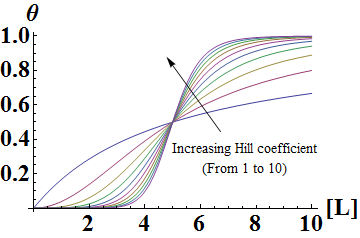
\includegraphics[width=.6\textwidth]{Hill_Graph.png}
        \label{fig:fighill}
    \end{figure}
\end{frame}

%------------------ %------------------ %------------------ %------------------ %------------------ %------------------ %------------------ 
% HERE WE RUN THROUGH A COUPLE OF FIGURES THAT DEMONSTRATE THE SYSTEM.
\section{Results}

\begin{frame}
    \begin{figure}[ht!]
        \centering
        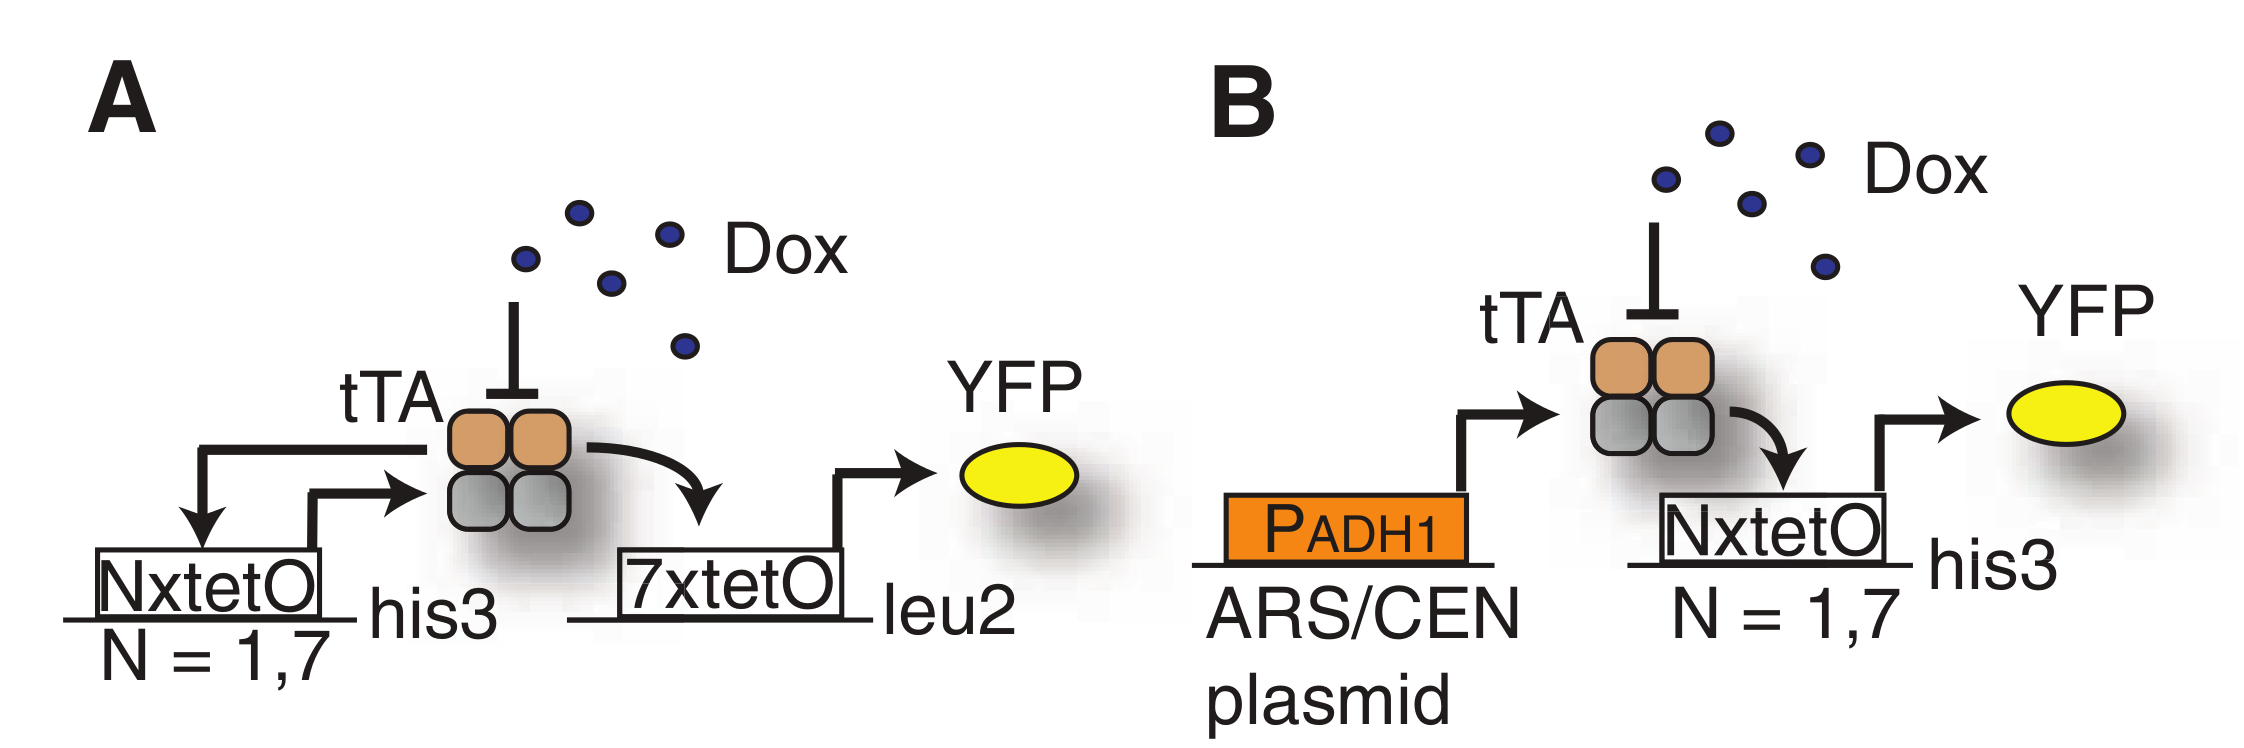
\includegraphics[width=.8\textwidth]{Tofig1b.png}
        \label{fig:fig1to}
    \end{figure}
    \begin{center}
        Closed-loop and open-loop systems
    \end{center}
\end{frame}


\begin{frame}
    % closed loop system
    \begin{figure}[ht!]
        \centering
        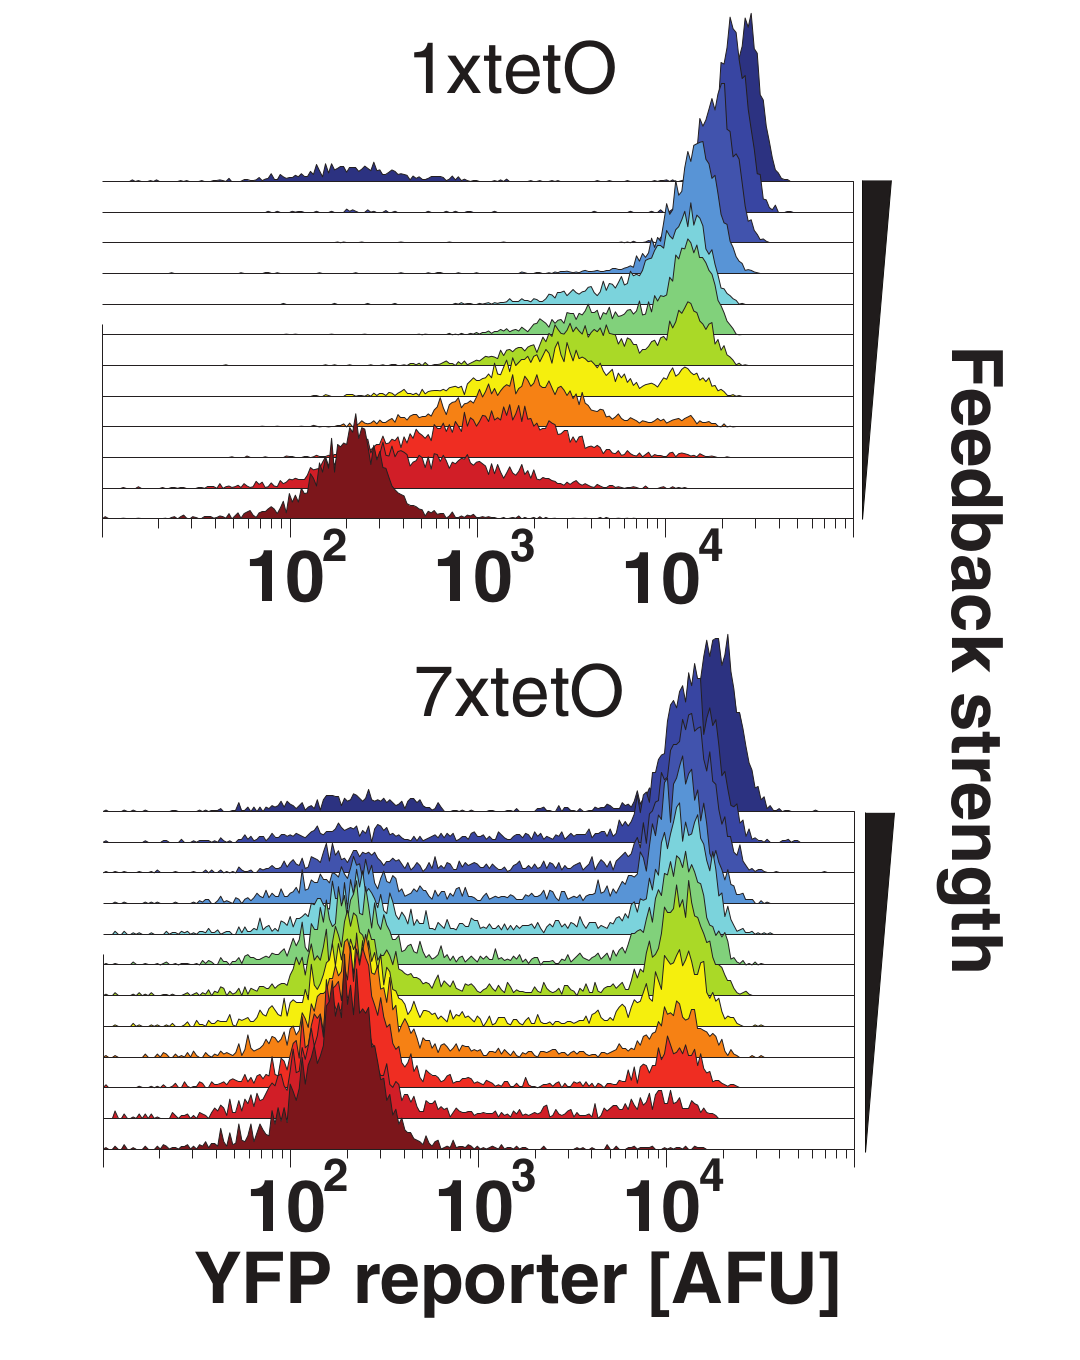
\includegraphics[width=.6\textwidth]{Tofig2.png}
        \label{fig:fig2to}
    \end{figure}
\end{frame}

\begin{frame}
    % The open-loop system
    \begin{figure}[ht!]
        \centering
        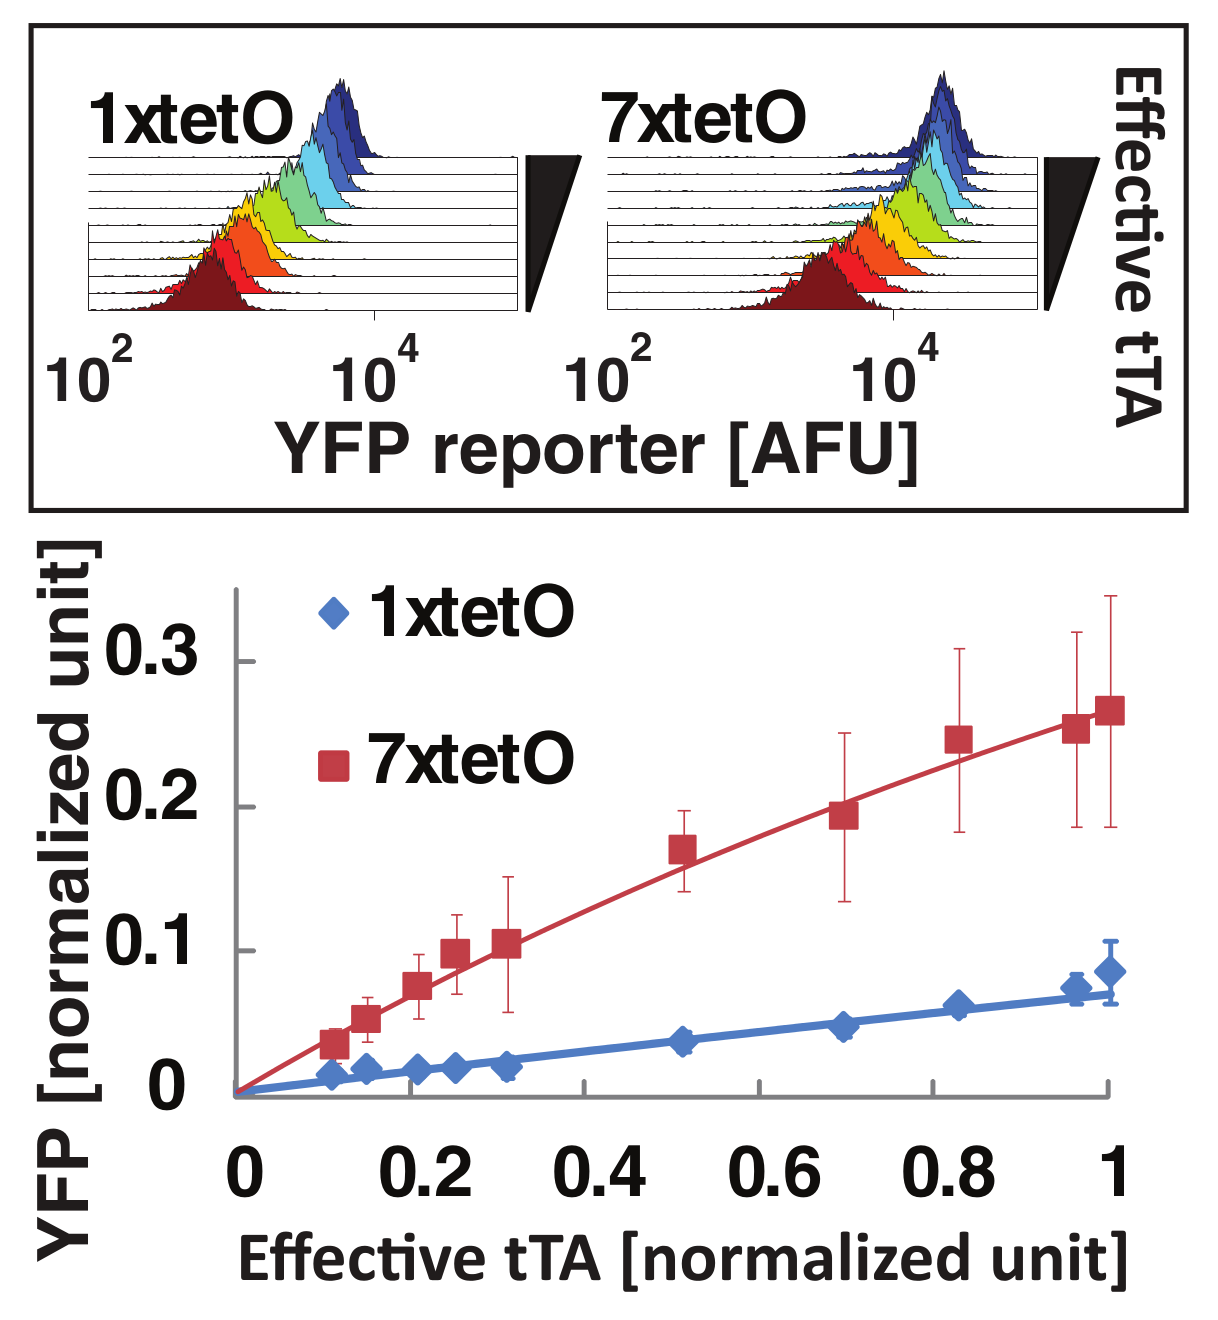
\includegraphics[width=.8\textwidth]{Tofig3.png}
        \label{fig:fig3to}
    \end{figure}
\end{frame}
  
 \begin{frame}
     % CAN NOISE INDUCE THIS BIMODALITY?? A SIMULATION.
    \begin{figure}[ht!]
        \centering
        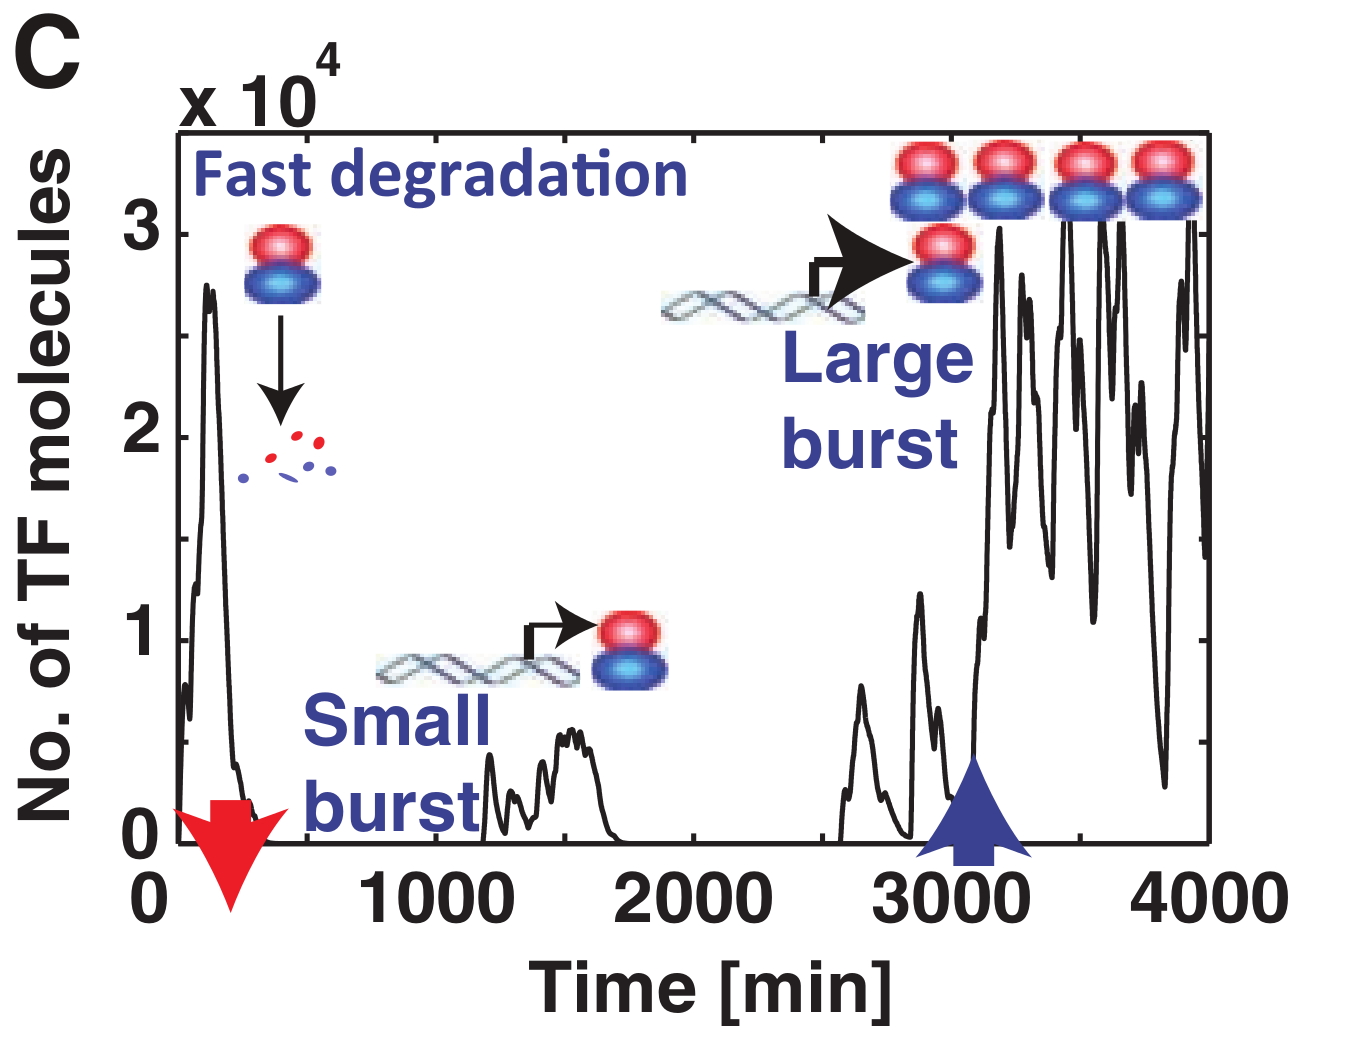
\includegraphics[width=.8\textwidth]{Tofig4.png}
        \caption{Simulation of transcriptional noise}
        \label{fig:fig4to}
    \end{figure}
\end{frame}

% hypothesized that the 7xtetO promoter had a
% lower maximum burst frequency and
% larger burst size versus the 1xtetO promoter.

 \begin{frame}
    \begin{figure}[ht!]
        \centering
        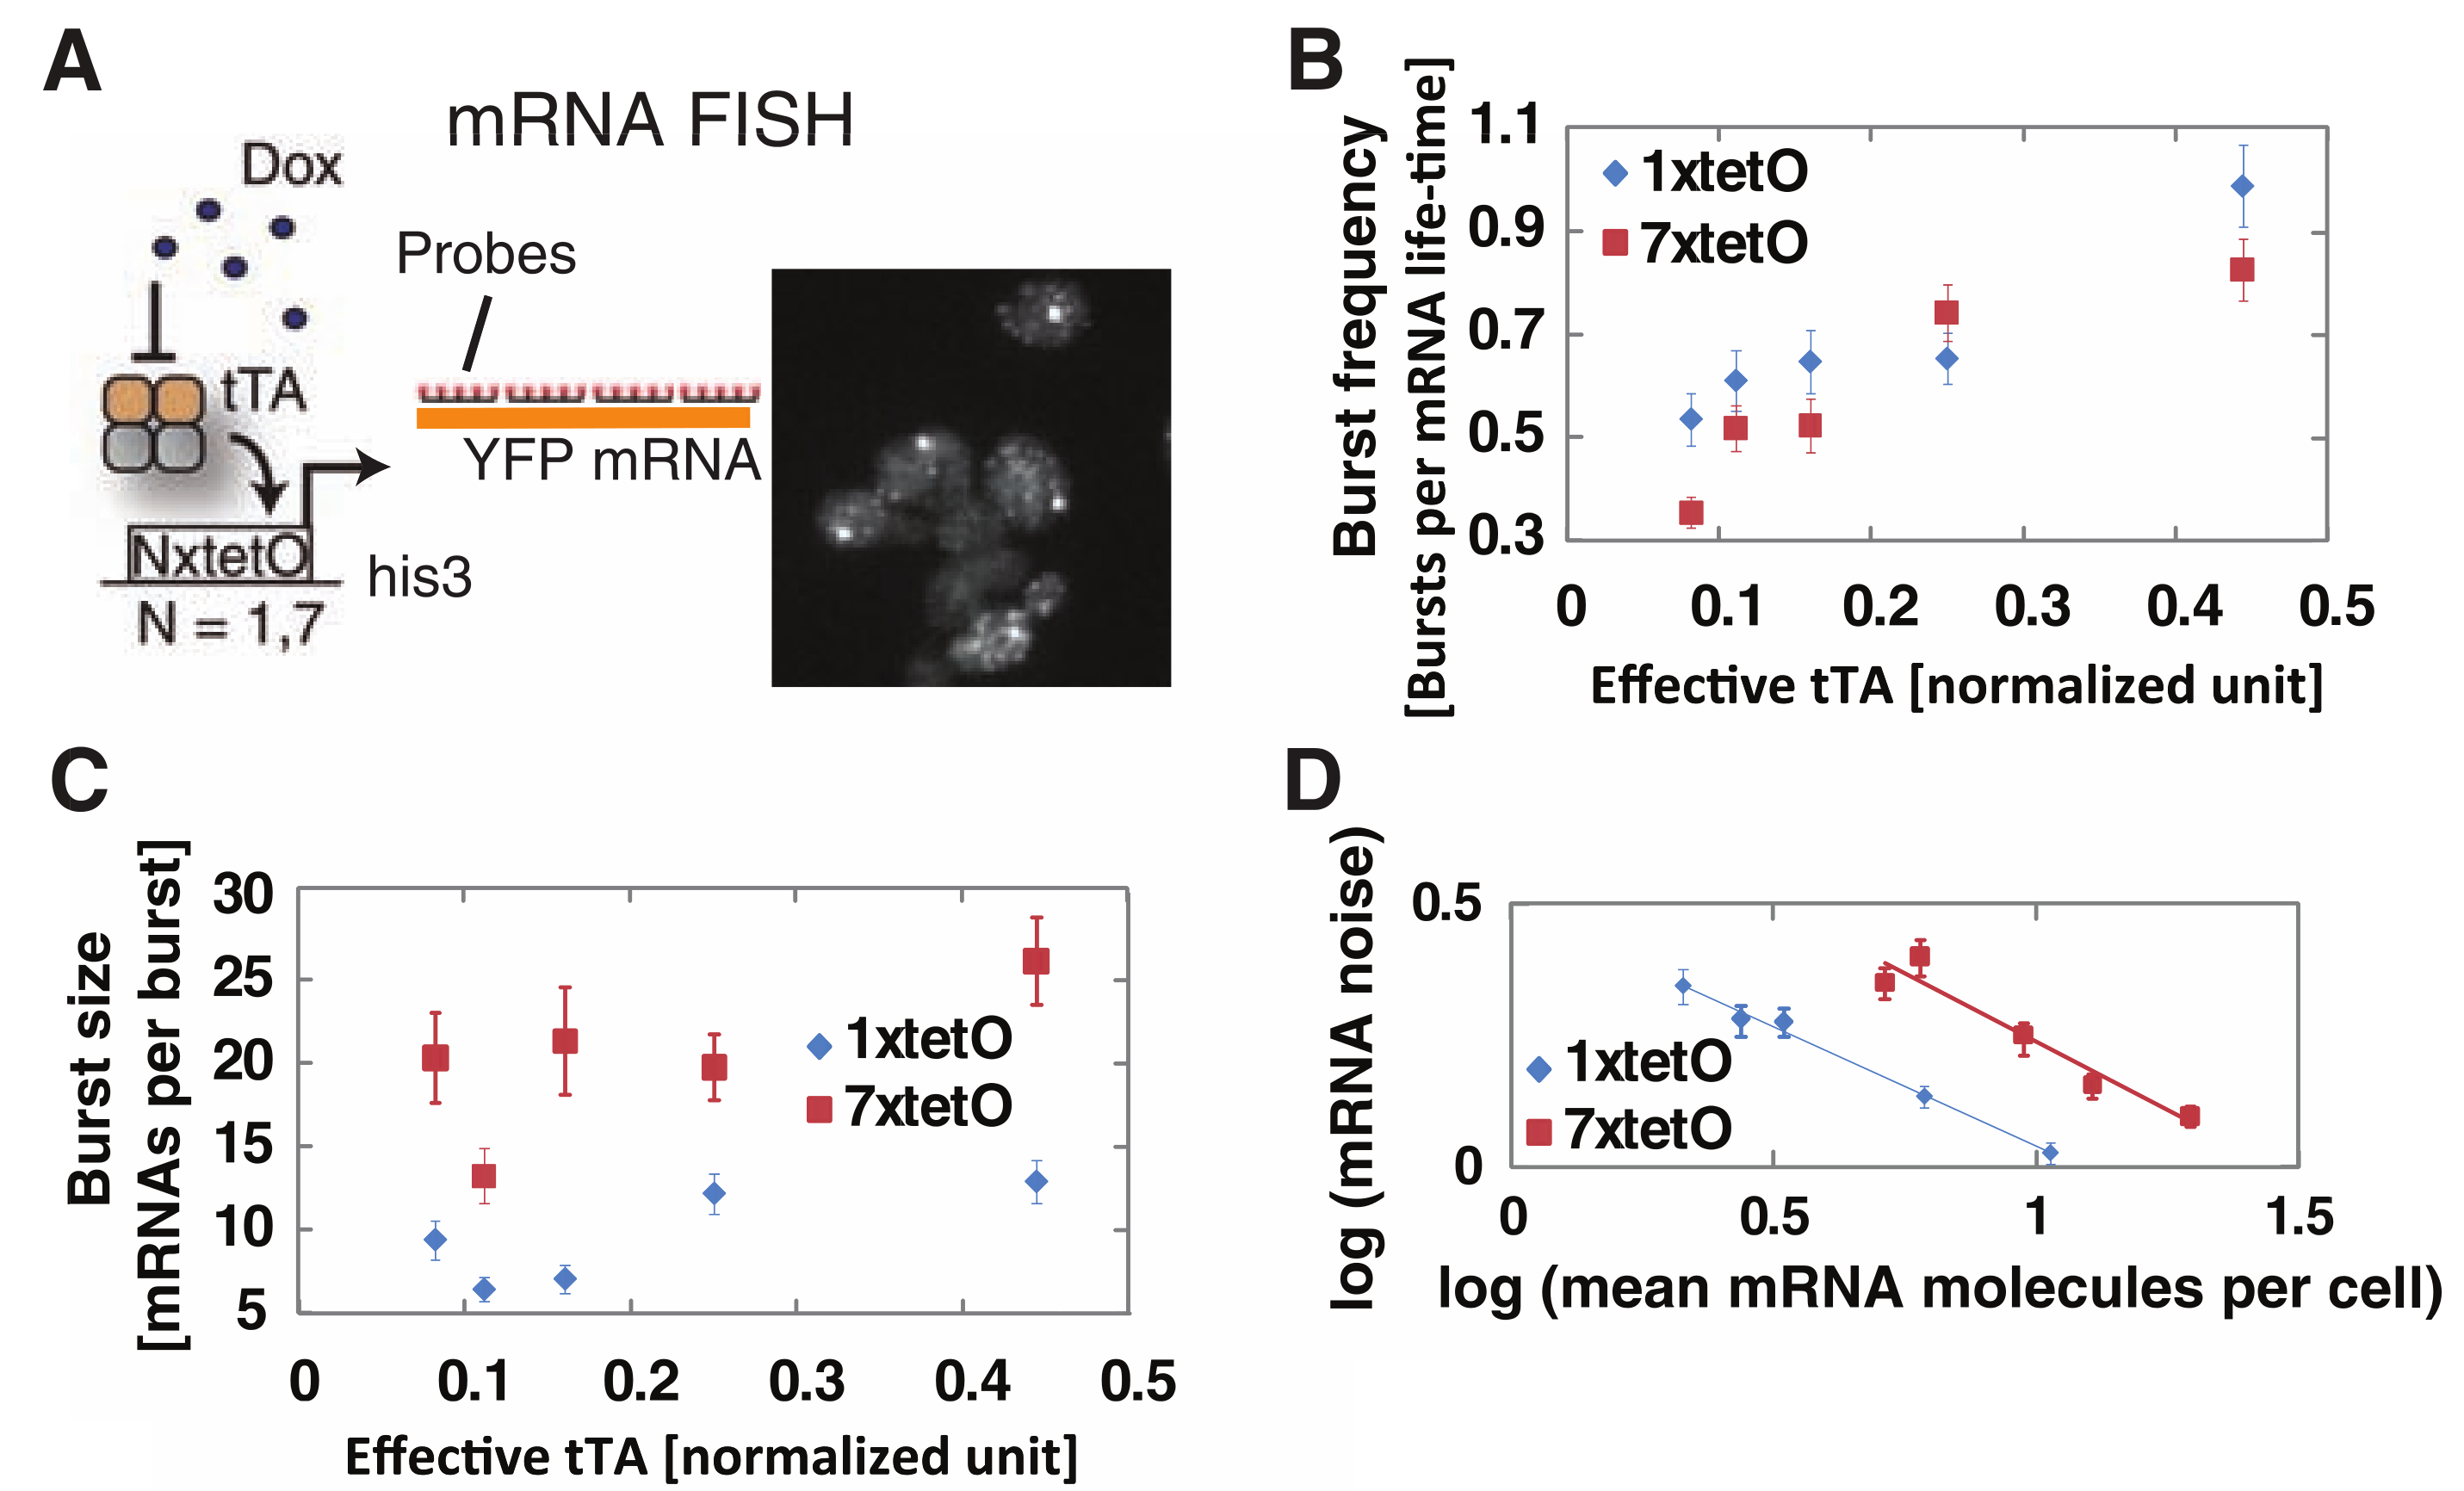
\includegraphics[width=.8\textwidth]{Tofig5.png}
        \label{fig:fig5to}
    \end{figure}
    \begin{figure}[ht!]
        \centering
        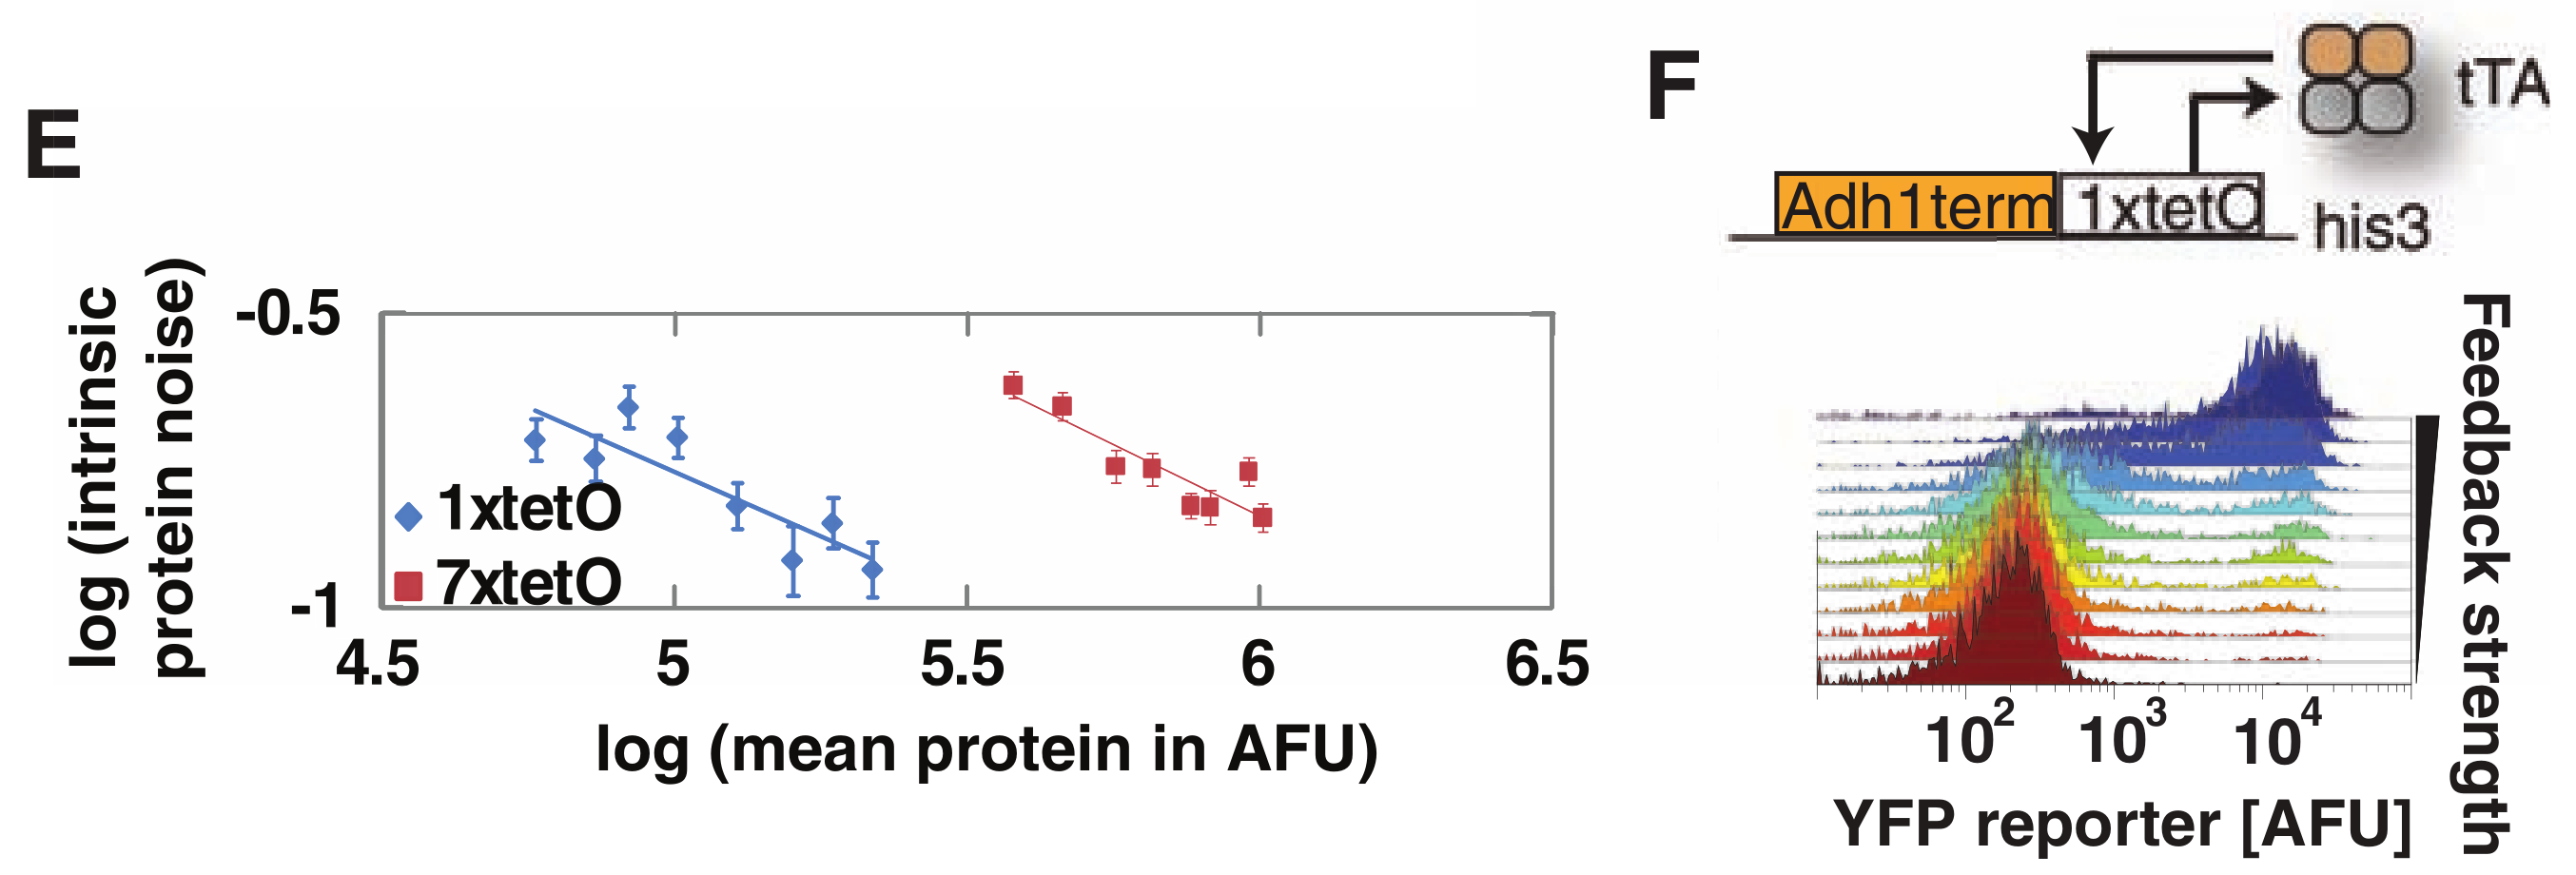
\includegraphics[width=.8\textwidth]{Tofig6.png}
        \label{fig:fig6to}
    \end{figure}
\end{frame}
 
 \begin{frame}
    \begin{figure}[ht!]
        \centering
        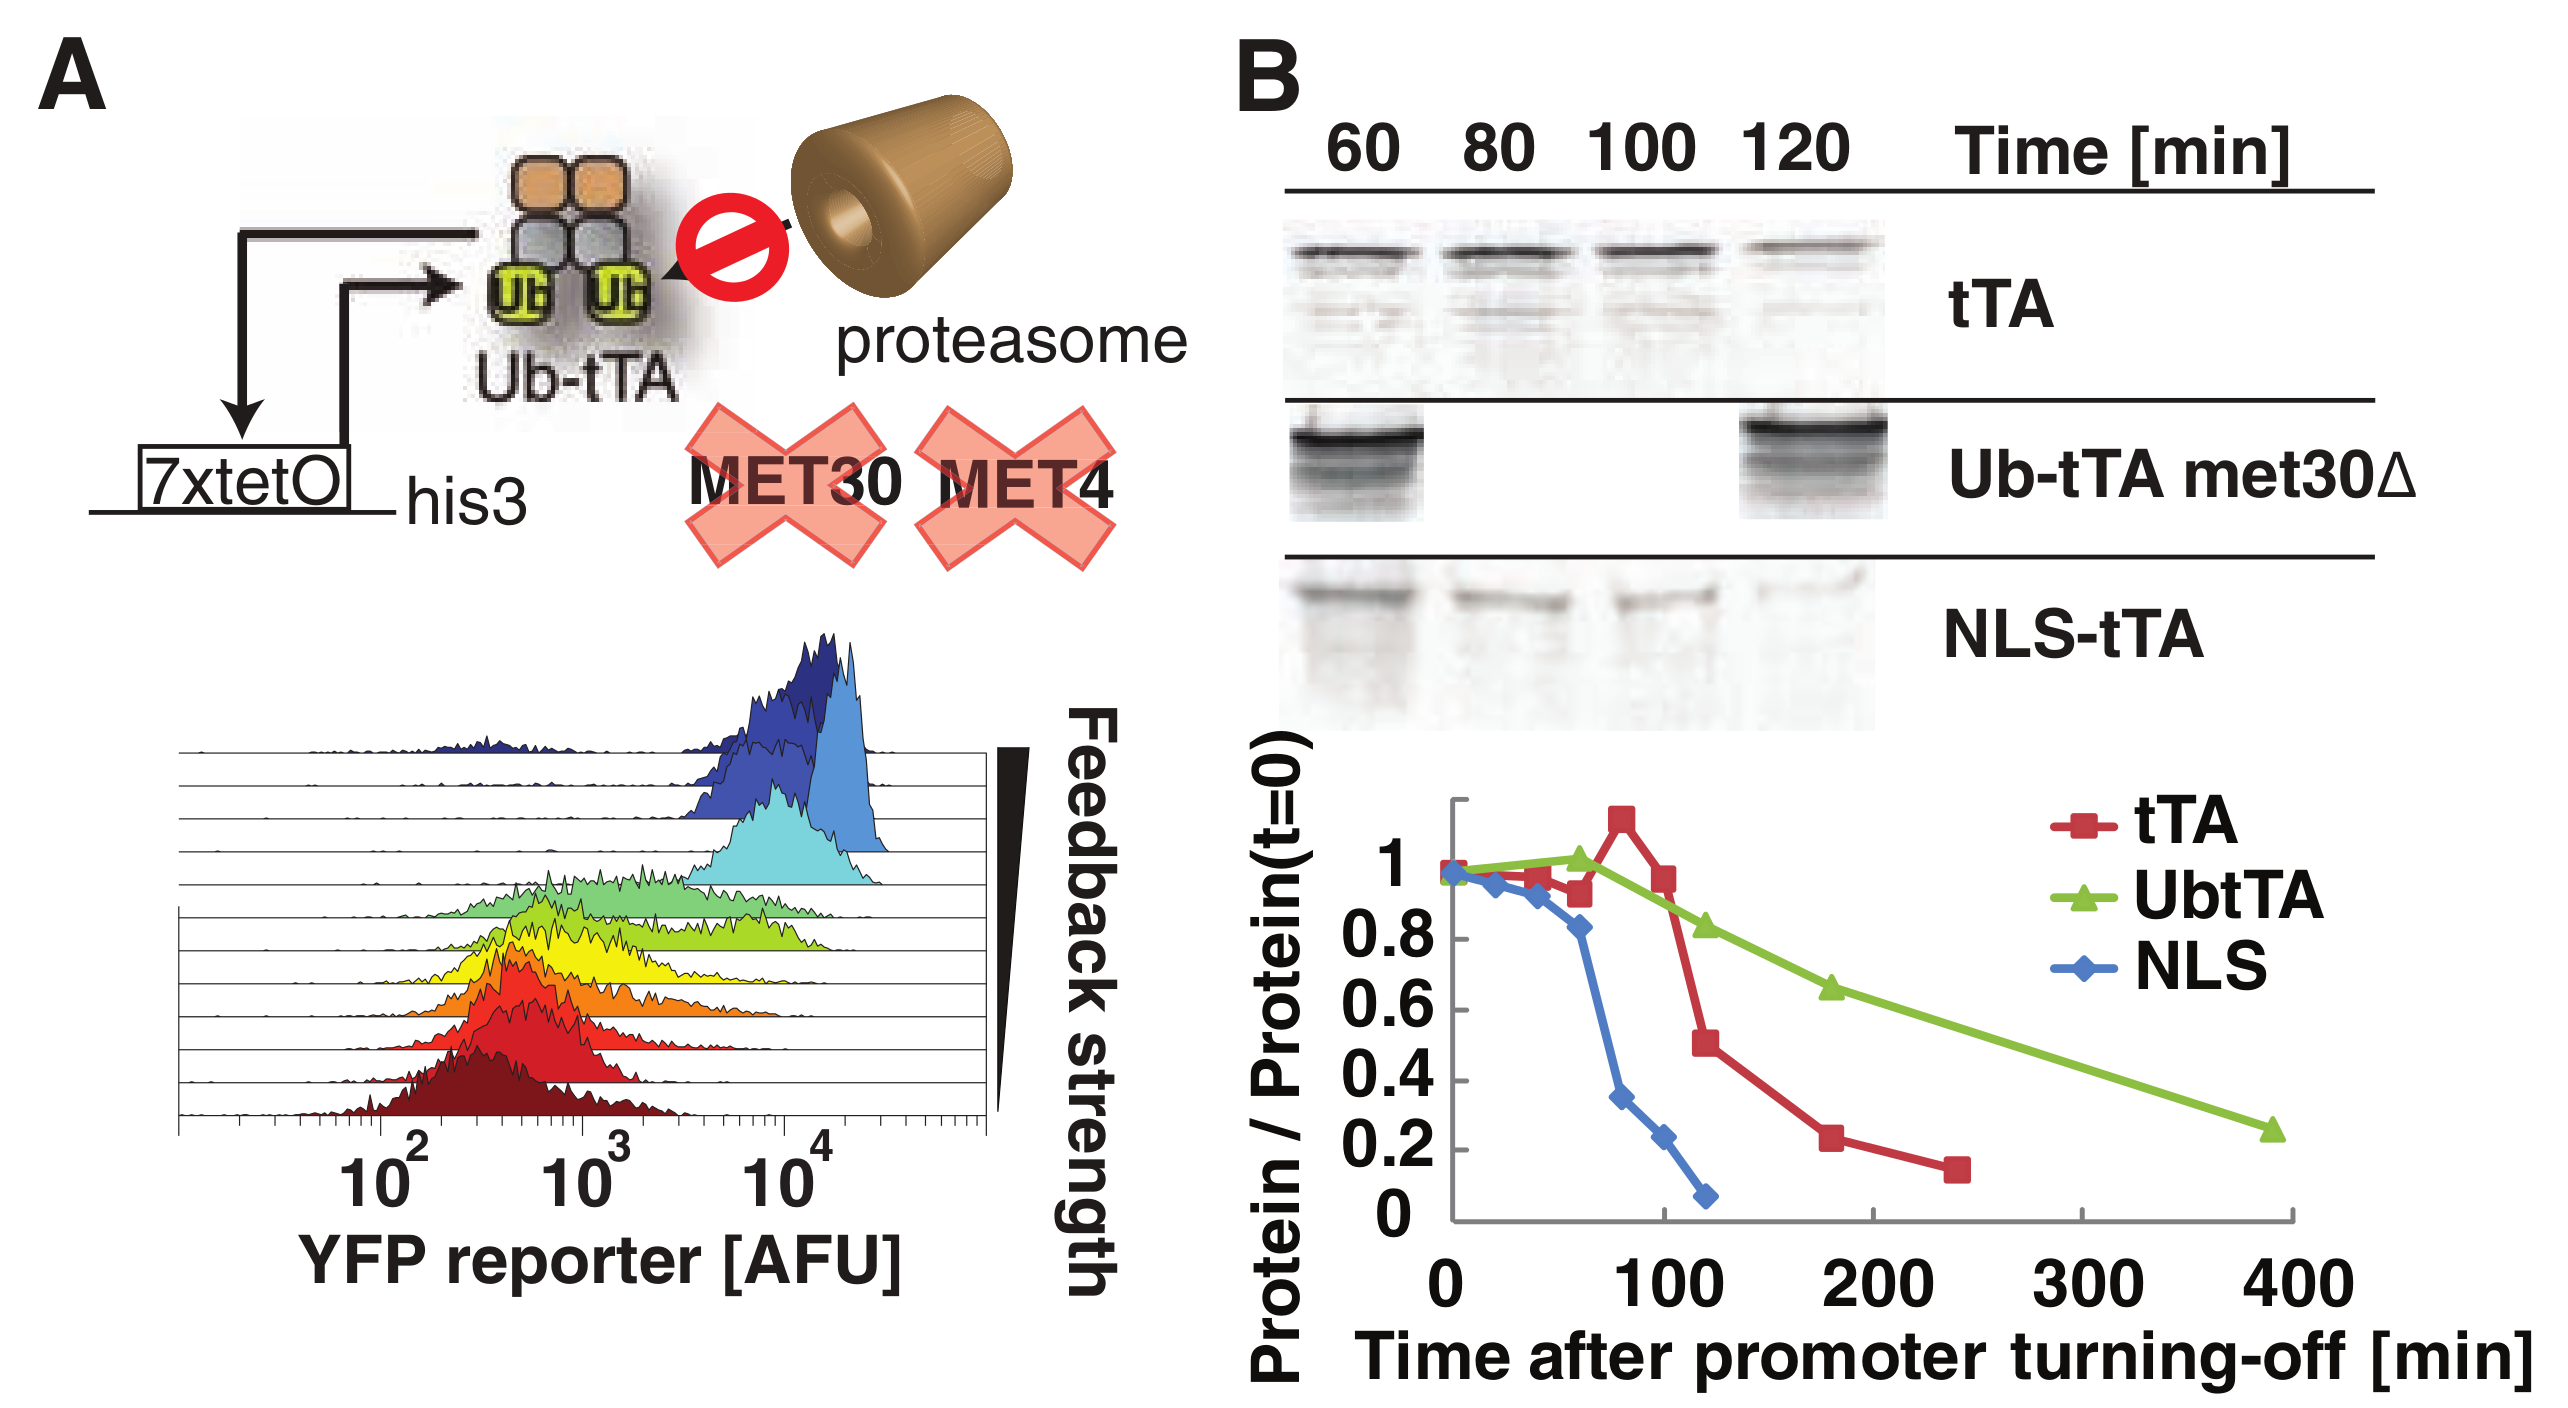
\includegraphics[width=.8\textwidth]{Tofig7.png}
        \caption{Test of model by stabilizing TF}
        \label{fig:fig7to}
    \end{figure}
\end{frame}
 
 \begin{frame}
    \begin{figure}[ht!]
        \centering
        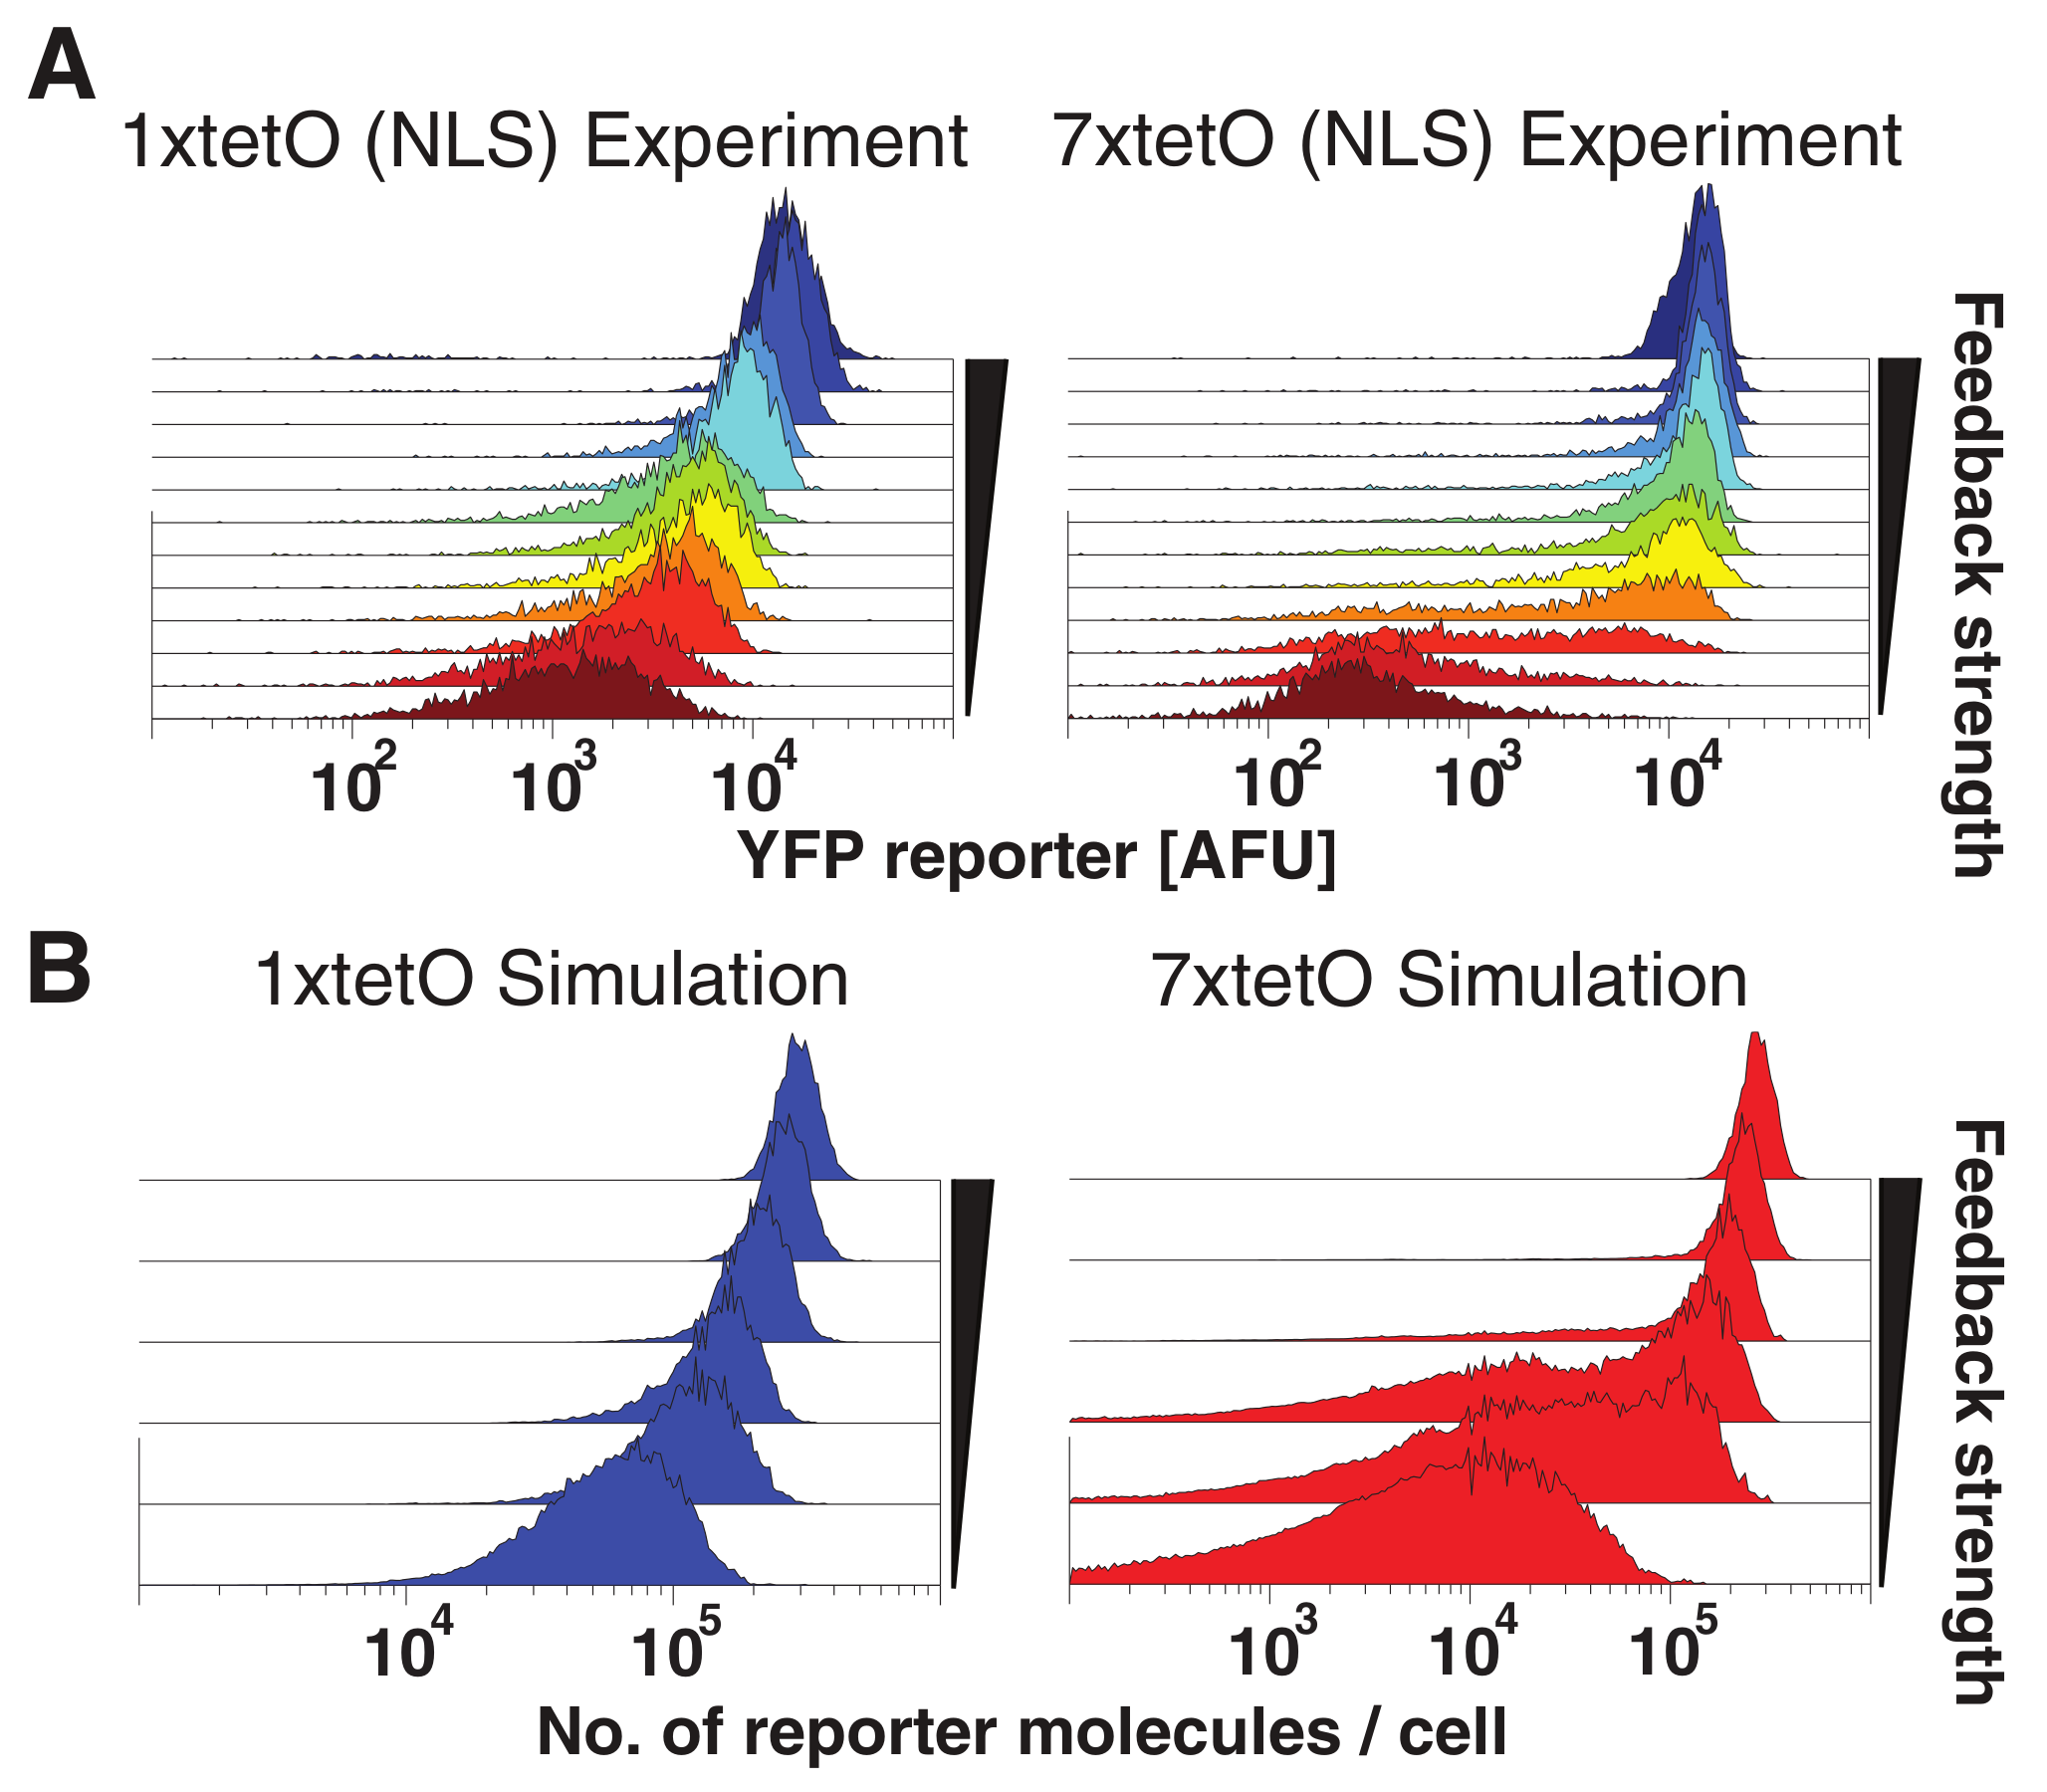
\includegraphics[width=.8\textwidth]{Tofig8.png}
        \label{fig:fig8to}
    \end{figure}
    % Localization + degradation.
\end{frame}

%------------------ %------------------ %------------------ %------------------ %------------------ %------------------ %------------------ 
\section{Conclusions}
\begin{frame}
    \begin{itemize}
        \item Noise can induce bimodality.
        \item System relies on having large and infrequent bursts of transcription.
        \item The 7xtetO has high sensitivity $\doubleleftarrow$ high noise.
        \item Can achieve this by having a unstable TF. For example, $t_{1/2} = \sim 15$ minutes.
    \end{itemize}
\end{frame}

\end{document}
